% THIS IS SIGPROC-SP.TEX - VERSION 3.1
% WORKS WITH V3.2SP OF ACM_PROC_ARTICLE-SP.CLS
% APRIL 2009
%
% It is an example file showing how to use the 'acm_proc_article-sp.cls' V3.2SP
% LaTeX2e document class file for Conference Proceedings submissions.
% ----------------------------------------------------------------------------------------------------------------
% This .tex file (and associated .cls V3.2SP) *DOES NOT* produce:
%       1) The Permission Statement
%       2) The Conference (location) Info information
%       3) The Copyright Line with ACM data
%       4) Page numbering
% ---------------------------------------------------------------------------------------------------------------
% It is an example which *does* use the .bib file (from which the .bbl file
% is produced).
% REMEMBER HOWEVER: After having produced the .bbl file,
% and prior to final submission,
% you need to 'insert'  your .bbl file into your source .tex file so as to provide
% ONE 'self-contained' source file.
%
% Questions regarding SIGS should be sent to
% Adrienne Griscti ---> griscti@acm.org
%
% Questions/suggestions regarding the guidelines, .tex and .cls files, etc. to
% Gerald Murray ---> murray@hq.acm.org
%
% For tracking purposes - this is V3.1SP - APRIL 2009

\documentclass{acm_proc_article-sp}

\usepackage{url}
\usepackage{listings}
\usepackage{graphicx}
\usepackage{fixltx2e}
\begin{document}

\numberofauthors{2} 
\author{
\alignauthor
Ivan Oropeza\\
       \affaddr{Dept. of Computer Science}\\
       \affaddr{University of Texas at Austin}\\
\alignauthor
William Xie\\
       \affaddr{Dept. of Computer Science}\\
       \affaddr{University of Texas at Austin}\\
}

\title{Hidden Markov Models vs. Maximum Entropy Markov Models}


\maketitle
\section{Introduction}
A frequent problem in many disciplines is the challenge to do sequence labelling. DNA sequencing, video semantic analysis, and Part-Of-Speech tagging are just some examples where sequence labelling is a crucial tasks that needs to be solved~\cite{dnaEx, videoEx, nlpEx}. In Natural Language Processing (NLP), Part-Of-Speech (POS) tagging is an stepping stone into solving more complex problems such as syntactic parsing of sentences. The typical techniques used to solve this problem are Hidden Markov Models (HMM), Maximum Entropy Markov Models (MEMM), and Conditional Random Fields (CRF). While CRFs are considered to be the state-of-the-art in POS tagging we want to compare the performance of the other models HMM and MEMM. This paper is structured in the following way: first we provide a brief description of the datasets used in this investigation. Then, we compare HMMs and MEMMs. Next, we discuss how the training process works for POS tagging. Finally, we compare the performance of HMMs vs MEMMs under similar situations.
\section{Datasets}
In this investigation we use the Wall Street Journal (WSJ), a 3-year collection of 2,499 articles from the Wall Street Journal. It has approximately 3 million words and was tagged by using statistically-based methods~\cite{wsjCorpus}. 

In addition to this corpus, we also use the Brown corpus. The Brown corpus is a collection of 500 text documents from 1961 sampled from various genres and sources ranging from fiction, press, and lore~\cite{brownCorpus}.
\section{HMM vs. MEM,}
A HMM is generative model for the joint distribution of states and observations. It follows a Markovian assumptions. The Markov assumption restricts the transitions between states to be dependent only on the immediate past~\cite{nlpBook}. On the other hand, MEMM is discriminative since it models the conditional probability of the state given the observation. 

An MEMM is an enhancement on the Maximum Entropy model, also known as a multinomial regression model which in turn attempts to do classification by making the fewest number of assumptions. Figure \ref{hmmVmemm} shows the pictorial differences between both graphical models. The added benefit of MEMMs over HMMs is that MEMMs are not limited to only modelling two aspects: $P( S_i | P_{i-1} )$ and $P( O_i | S_i )$. Instead, MEMMs consider information derived directly from features applied on the observation in addition to the previous state knowledge. For example, capitalization often occurs with Nouns and specific suffixes such as "ed" and "ing" tend to be associated with Verbs are some useful features that can not be modelled by an HMM but can be modelled by an MEMM. Moreover, the typical algorithm used to solve the decoding problem in an HMM can be trivially modified to solve the decoding problem in an MEMM without additional overhead~\cite{nlpBook}.
\begin{figure}[ht]
\centering
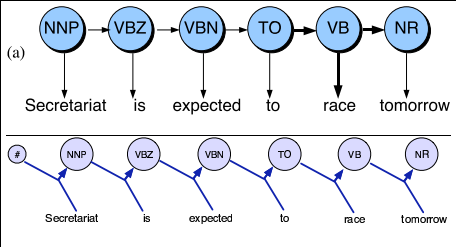
\includegraphics[width=80mm]{figures/memm.png}
\caption{Hidden Markov Model(top) and Maximum Entropy Markov Model(bottom)~\cite{nlpBook} \label{hmmVmemm}}
\end{figure}

\section{Learning}

\bibliographystyle{abbrv}
\bibliography{references}
\end{document}
